\section{Introduction}
\label{introduction}

GPUs have revolutionized and massively transformed the high
performance computing, machine learning, and data analytics landscapes that were
previously dominated by CPU-based
installations~\cite{pascal,intersect360,cudnn,Lavin15b,SimonyanZ14a}. Modern
computing systems rely on combination of GPUs and CPUs to leverage high
throughput data parallel GPUs in combination with the traditional benefits of
latency critical serial execution on CPUs. GPU-accelerated computing has been
naturally successful in these domains because of its native support for data parallel
programming languages~\cite{CUDA7,OPENCL} that reduces programmer burden when
trying to scale their programs across ever growing data sets.

\begin{figure}[t]
\centering
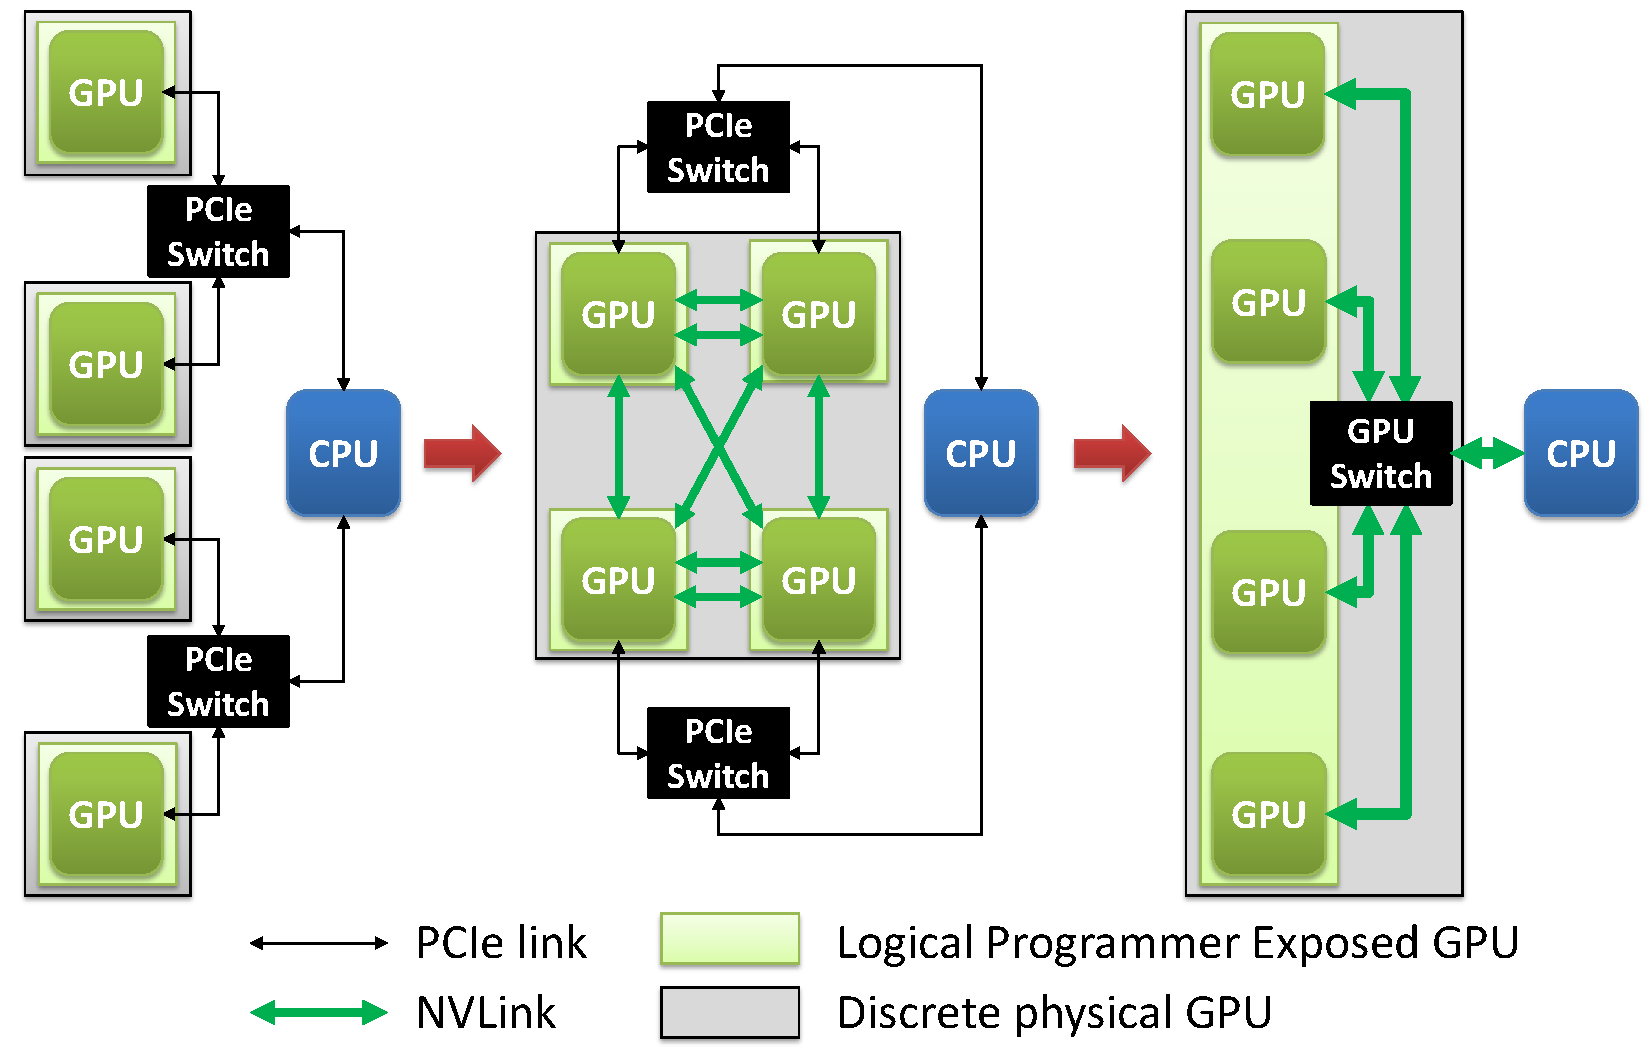
\includegraphics[width=1.0\columnwidth]{figures/inter_gpu_connections.pdf}
\caption{The evolution of GPUs from discrete pluggable PCIe devices to high pin-count 
multi-socket accelerators utilizing switched interconnects.}
\label{fig:systemdiagram}
\vspace{-.15in}
\end{figure}

Nevertheless, with GPU dies nearing the reticle limitation for maximal die size, and transistor
density growth rate slowing down~\cite{mooredead2016}, programmers looking to
scale the performance of their programs on a single-GPU are in a precarious
position. Multi-GPU programming models support explicit programming of multiple GPUs,
nevertheless it is still a very challenging task requiring unique programming skills
along with leveraging special mechanisms such as Peer-2-Peer
access~\cite{NVIDIAP2P}, or a combination of MPI and CUDA~\cite{NVIDIAMPI} to
manage multiple GPUs. These programming extensions enable advanced programmers
to leverage more than one GPU for high throughput computation but require
re-writing of the single-GPU application, which may slow its adoption rate. 

Recently GPUs have started making the transition from using the PCIe peripheral 
interface to having improved interconnections between both the GPUs and 
CPUs~\cite{dgx,AMDINFINITYFABRIC} as shown in Figure~\ref{fig:systemdiagram}. 
This way GPUs evolved from being a discrete pluggable PCIe accelerator into a
first-class system component using a high pin-count socket very similar to
modern CPU interfaces.
This socket interface is required not only for power delivery, 
but because the GPU and CPU interconnects require printed
circuit board (PCB) level integration to provide its massive interconnect bandwidth.
This evolution of GPUs from single socket, to high connectivity multi-socket designs
is a natural progression when trying to improve intra-GPU communication.

Multi-socket GPUs provide a pivot point for GPU and system vendors. On one hand, they
could continue to expose multi-socket GPUs as discrete GPUs and force programmers
to re-write their applications to try and improve scaling beyond a single socket.
On the other hand, they could now choose to expose these multi-socket designs as
a single non-uniform memory access (NUMA) GPU resource. The later solution allows 
significant performance scaling beyond the single GPU transistor growth, all
while maintaining the single-GPU programming model GPU developers have standardized upon.

We are not the first group to propose that there may be potential performance
benefits to aggregating GPUs together, without changing programming
interface~\cite{Cabezas2015,lee2013transparent}. However, much of this work was
done in an era where GPUs were limited in the memory they could address in the
system and high latency PCIe interconnects were the standard interconnect
technology. These restrictions cause prior work to primarily focus on improving
programming and runtime interfaces when trying to aggregate multiple discrete
GPUs. In this work we propose that in the era of unified virtual addressing,
cache line addressable high bandwidth interconnects, and dedicated CPU--GPU
socketed PCB designs, multi-socket GPUs should be treated as single NUMA-GPUs
and their microarchitectures need to be optimized to maximize multi-socket GPU
performance.

In this work we examine an evolutionary multi-socket GPU system and describe the 
basic architectural modifications needed to allow this multi-socket GPU system to appear to the programmer
as single large GPU, obeying all of the current GPU programming paradigms. We apply 
several well known NUMA techniques from the CPU world and show that
while having a positive effect, simply applying CPU NUMA design principles to GPUs 
will be insufficient. Thus we propose that to design
a single program scalable multi-GPU system, GPU architectures themselves must become
\textit{NUMA-aware} to handle the NUMA effects that are implicit in a multi-socket
design. In this work, we make the following contributions:

\begin{enumerate}
\item
We show that despite being highly data parallel, GPU programs have significant
dynamic phase behavior both between kernels and among CTAs within a single
kernel that should be microarchitecturally exploited to eliminate observed
NUMA effects.

\item
We demonstrate that traditionally used symmetric and statically assigned inter-GPU link bandwidth allocations 
limit multi-GPU scalability in many cases. We propose
that GPU interconnects need to support dynamic bandwidth balancing that can
turn around $N$ of $M$ high speed serial links at run time to support asymmetric
bandwidth settings. We demonstrate that our dynamic policy is coarse
grained enough that the performance improvement is largely insensitive to link turn 
around and policy sample time. Moreover, we show that dynamic policies must be on a
per GPU basis, as unified global policies fail to capture per GPU locality
resulting in suboptimal performance.

\item
Our findings indicate that simple extension of GPUs SW-based L1s coherency into
L2 caches in multi-socket GPU scenario will be sub-optimal.  
We examine the trade-offs of such a coherency scheme in detail, 
along with several cache partitioning and allocation policies that trade-off
caching efficiency with invalidation overheads. We show that with minor modifications, 
current GPU coherence protocols can perform well in properly architected multi-GPU caches.

\item Finally, we show that architecting a single static cache architecture for
multi-GPUs yields a sub-optimal performance. We demonstrate that re-balancing cache
capacity between local and remote accesses in multi-socket GPU systems is
required both on a per workload basis, but also a per socket basis to leverage
applications phase behavior. We develop a mechanisms that allows cache capacity
to be dynamically reallocated to compensate for constantly changing bandwidth
bottlenecks and help mitigate NUMA effects in multi-socket GPUs.

% Dynamic cache partitioning: given that different benchmarks prefer different 
% cache configurations, we evaluate dynamic way-partitioning of gpu-side L2 
% caches. Depending on local and remote BW saturations, we adjust the number of 
% ways reserved for caching local and remote data. Alone, this mechanism improves 
% the performance by X% and we are within Y% of 1x gpu-side RC + 1x mem-side L2. 
% Combined with dynamic NVLink balancing, we improve the performance by Z% over 
% the baseline TMG and we are within ZZ% of 2x NVlink + 1x gpu-side + 1x mem-side 
% L2. Finally, this increases the scalability compared to a single-GPU system by 
% YY%.




% 
% General story about increasing the performance by putting multiple GPUs working 
% together (TMG). No code re-writing, no re-compilation, what can we expect if we 
% just allow the runtime to distribute CTAs across multiple GPUs?
% With CUDA providing UVAS and UMA, and NVLink supporting atomic , GPU-NUMA system 
% is born: there is ~10x difference between local and remote BW (local mem 
% BW=1TB/s and NVLink BW is 128GB/s) which limits the scalability and stands as a 
% bottleneck. It is not about latency, it is about BW. (maybe some nvlink latency 
% vs bw graph here?). The question is what can we do from the micro-arch side to 
% improve this?

% Technology trends indicate an increasing number of systems designed with CPUs, 
% accelerators, and GPUs coupled via high-speed 
% links. Such systems are likely to introduce unified shared
% CPU-GPU memory with shared page tables. In fact, some systems already
% feature such implementations~\cite{AMDKaveri}.
% Introducing globally visible shared memory
% improves programmer productivity by eliminating explicit copies and memory 
% management overheads. Whereas this abstraction can be supported using
% software-only page-level protection mechanisms~\cite{UVM, HSA}, hardware cache coherence 
% can improve performance by allowing concurrent, fine-grained access to memory
% by both CPU and GPU.  If the CPU and GPU have separate physical
% memories, page migration may also be used to optimize page placement for
% latency or bandwidth by using both near and far 
% memory~\cite{Dashti2013,Agarwal2015b,Meswani2015,Chou2015}.
% 
% 
% 
% Some CPU--GPU systems will be tightly integrated into a system on chip (SoC) making on-chip 
% hardware coherence a natural fit, possibly even by sharing a portion of the on-chip 
% cache hierarchy~\cite{HSA,AMDAPU,Hechtman2014}.  However, the largest GPU 
% implementations consume nearly 8B transistors and have their own 
% specialized memory systems~\cite{NVIDIA8BILLION}.  
% Power and thermal constraints preclude single-die integration of such designs. 
% Thus, many CPU--GPU systems are likely to have 
% discrete CPUs and GPUs connected via dedicated off-chip interconnects like 
% NVLINK (NVIDIA), CAPI (IBM), HT (AMD), and QPI (INTEL) or implemented as 
% multi-chip modules~\cite{NVLINK,CAPI,AMDHT,INTELQPI,Chen92}. The availability of these
% high speed off-chip interconnects has led both academic groups and vendors like NVIDIA
% to investigate how future GPUs may integrate into existing OS-controlled 
% unified shared memory regimes used by CPUs~\cite{Pichai2014,power2014,Agarwal2015,Agarwal2015b}.
% 
% Current CPUs have up to 18 cores per socket~\cite{INTELXEONE5V3} but GPUs are 
% expected to have hundreds of streaming multiprocessors (SMs) each with its own cache(s) within 
% the next few years. Hence, extending traditional hardware cache-coherency into a multi-chip 
% CPU--GPU memory system requires coherence messages to be exchanged not just within the GPU but
% over the CPU--GPU interconnect. Keeping these hundreds of caches coherent with a traditional HW
% coherence protocol, as shown in
% Figure~\ref{fig:motivation}, potentially requires large state and interconnect 
% bandwidth~\cite{Kelm2010,johnson2011}. 
% Some recent proposals call for heterogeneous race-free (HRF) GPU programming models, which
% allow relaxed or scoped memory consistency to reduce the frequency or hide the
% latency of enforcing coherence~\cite{Hechtman2014}. 
% Others argue that scopes substantially increase programmer burden, and instead propose
% a data-race-free programming model with coherence based on reader-initiated invalidation~\cite{Sinclair2015}.
% However, irrespective of 
% memory ordering requirements, such approaches either require software to initiate flushes
% at synchronization points or system-wide hardware cache coherence mechanisms.
% We show
% that Selective Caching can achieve performance rivaling
% more complex CPU-GPU cache coherence protocols.
% Techniques like region coherence~\cite{Power2013} 
% seek to scale coherence protocols for heterogeneous systems, but require
% pervasive changes throughout the CPU and GPU memory systems. Such approaches
% also incur highly coordinated design and verification effort by both CPU and GPU
% vendors~\cite{Hong2012} that is challenging when multiple vendors wish to integrate
% existing CPU and GPU designs in a timely manner.
% 
% In the past, NVIDIA has investigated extending hardware cache-coherence 
% mechanisms to multi-chip CPU--GPU memory systems. Due to the significant challenges
% associated with building such systems, in this work, we architect a GPU \textit{selective caching} 
% mechanism. This mechanism provides the conceptual simplicity of CPU--GPU hardware cache coherence and
% maintains a high level of GPU performance, but does not actually implement
% hardware cache coherence within the GPU, or between the CPU and GPU. In our proposed 
% selective caching GPU, the GPU does not cache data that resides in CPU physical 
% memory, nor does it cache data that resides in the GPU memory that is 
% actively in-use by the CPU on-chip caches. This approach is orthogonal to the memory
% consistency model and leverages the latency-tolerant nature of GPU architectures combined with upcoming low-latency and 
% high-bandwidth interconnects to enable the benefits of shared memory.  To evaluate the performance
% of such a GPU, we measure ourselves against a theoretical hardware
% cache-coherent CPU--GPU system that, 
% while high performance, is impractical to implement.
% 
% In this work, we make the following contributions:
% 
% \begin{enumerate}
% % \vspace{-.05in}
% \item
% We propose GPU selective caching, which enables a CPU--GPU system that provides a 
% unified shared memory without requiring hardware cache-coherence protocols within the GPU
% or between CPU and GPU caches.
% % \vspace{-.05in}
% \item
% We identify that much of the improvement from GPU caches is due to coalescing 
% memory accesses that are spatially contiguous.  Leveraging
% aggressive request coalescing, GPUs can achieve much of the performance benefit
% of caching, without caches.
% % \vspace{-.05in}
% \item
% We propose a small on-die CPU cache to handle uncached GPU requests
% that are issued at sub-cache line granularity. This cache helps both 
% shield the CPU memory system from the bandwidth hungry GPU and supports
% improved CPU--GPU interconnect efficiency by implementing variable-sized transfer granularity.
% % \vspace{-.05in}
% \item
% We demonstrate that a large fraction of GPU-accessed data is read-only. Allowing 
% the GPU to cache this data and relying on page protection mechanisms rather than hardware 
% coherence to ensure correctness closes the performance gap between a selective
% caching and hardware cache-coherent GPU for many applications.
% % \vspace{-.05in}
\end{enumerate}
